\documentclass[]{book}
\usepackage{lmodern}
\usepackage{amssymb,amsmath}
\usepackage{ifxetex,ifluatex}
\usepackage{fixltx2e} % provides \textsubscript
\ifnum 0\ifxetex 1\fi\ifluatex 1\fi=0 % if pdftex
  \usepackage[T1]{fontenc}
  \usepackage[utf8]{inputenc}
\else % if luatex or xelatex
  \ifxetex
    \usepackage{mathspec}
  \else
    \usepackage{fontspec}
  \fi
  \defaultfontfeatures{Ligatures=TeX,Scale=MatchLowercase}
\fi
% use upquote if available, for straight quotes in verbatim environments
\IfFileExists{upquote.sty}{\usepackage{upquote}}{}
% use microtype if available
\IfFileExists{microtype.sty}{%
\usepackage{microtype}
\UseMicrotypeSet[protrusion]{basicmath} % disable protrusion for tt fonts
}{}
\usepackage[margin=1in]{geometry}
\usepackage{hyperref}
\hypersetup{unicode=true,
            pdftitle={R Lab for Regression Analysis},
            pdfborder={0 0 0},
            breaklinks=true}
\urlstyle{same}  % don't use monospace font for urls
\usepackage{natbib}
\bibliographystyle{apalike}
\usepackage{color}
\usepackage{fancyvrb}
\newcommand{\VerbBar}{|}
\newcommand{\VERB}{\Verb[commandchars=\\\{\}]}
\DefineVerbatimEnvironment{Highlighting}{Verbatim}{commandchars=\\\{\}}
% Add ',fontsize=\small' for more characters per line
\usepackage{framed}
\definecolor{shadecolor}{RGB}{248,248,248}
\newenvironment{Shaded}{\begin{snugshade}}{\end{snugshade}}
\newcommand{\AlertTok}[1]{\textcolor[rgb]{0.94,0.16,0.16}{#1}}
\newcommand{\AnnotationTok}[1]{\textcolor[rgb]{0.56,0.35,0.01}{\textbf{\textit{#1}}}}
\newcommand{\AttributeTok}[1]{\textcolor[rgb]{0.77,0.63,0.00}{#1}}
\newcommand{\BaseNTok}[1]{\textcolor[rgb]{0.00,0.00,0.81}{#1}}
\newcommand{\BuiltInTok}[1]{#1}
\newcommand{\CharTok}[1]{\textcolor[rgb]{0.31,0.60,0.02}{#1}}
\newcommand{\CommentTok}[1]{\textcolor[rgb]{0.56,0.35,0.01}{\textit{#1}}}
\newcommand{\CommentVarTok}[1]{\textcolor[rgb]{0.56,0.35,0.01}{\textbf{\textit{#1}}}}
\newcommand{\ConstantTok}[1]{\textcolor[rgb]{0.00,0.00,0.00}{#1}}
\newcommand{\ControlFlowTok}[1]{\textcolor[rgb]{0.13,0.29,0.53}{\textbf{#1}}}
\newcommand{\DataTypeTok}[1]{\textcolor[rgb]{0.13,0.29,0.53}{#1}}
\newcommand{\DecValTok}[1]{\textcolor[rgb]{0.00,0.00,0.81}{#1}}
\newcommand{\DocumentationTok}[1]{\textcolor[rgb]{0.56,0.35,0.01}{\textbf{\textit{#1}}}}
\newcommand{\ErrorTok}[1]{\textcolor[rgb]{0.64,0.00,0.00}{\textbf{#1}}}
\newcommand{\ExtensionTok}[1]{#1}
\newcommand{\FloatTok}[1]{\textcolor[rgb]{0.00,0.00,0.81}{#1}}
\newcommand{\FunctionTok}[1]{\textcolor[rgb]{0.00,0.00,0.00}{#1}}
\newcommand{\ImportTok}[1]{#1}
\newcommand{\InformationTok}[1]{\textcolor[rgb]{0.56,0.35,0.01}{\textbf{\textit{#1}}}}
\newcommand{\KeywordTok}[1]{\textcolor[rgb]{0.13,0.29,0.53}{\textbf{#1}}}
\newcommand{\NormalTok}[1]{#1}
\newcommand{\OperatorTok}[1]{\textcolor[rgb]{0.81,0.36,0.00}{\textbf{#1}}}
\newcommand{\OtherTok}[1]{\textcolor[rgb]{0.56,0.35,0.01}{#1}}
\newcommand{\PreprocessorTok}[1]{\textcolor[rgb]{0.56,0.35,0.01}{\textit{#1}}}
\newcommand{\RegionMarkerTok}[1]{#1}
\newcommand{\SpecialCharTok}[1]{\textcolor[rgb]{0.00,0.00,0.00}{#1}}
\newcommand{\SpecialStringTok}[1]{\textcolor[rgb]{0.31,0.60,0.02}{#1}}
\newcommand{\StringTok}[1]{\textcolor[rgb]{0.31,0.60,0.02}{#1}}
\newcommand{\VariableTok}[1]{\textcolor[rgb]{0.00,0.00,0.00}{#1}}
\newcommand{\VerbatimStringTok}[1]{\textcolor[rgb]{0.31,0.60,0.02}{#1}}
\newcommand{\WarningTok}[1]{\textcolor[rgb]{0.56,0.35,0.01}{\textbf{\textit{#1}}}}
\usepackage{longtable,booktabs}
\usepackage{graphicx,grffile}
\makeatletter
\def\maxwidth{\ifdim\Gin@nat@width>\linewidth\linewidth\else\Gin@nat@width\fi}
\def\maxheight{\ifdim\Gin@nat@height>\textheight\textheight\else\Gin@nat@height\fi}
\makeatother
% Scale images if necessary, so that they will not overflow the page
% margins by default, and it is still possible to overwrite the defaults
% using explicit options in \includegraphics[width, height, ...]{}
\setkeys{Gin}{width=\maxwidth,height=\maxheight,keepaspectratio}
\IfFileExists{parskip.sty}{%
\usepackage{parskip}
}{% else
\setlength{\parindent}{0pt}
\setlength{\parskip}{6pt plus 2pt minus 1pt}
}
\setlength{\emergencystretch}{3em}  % prevent overfull lines
\providecommand{\tightlist}{%
  \setlength{\itemsep}{0pt}\setlength{\parskip}{0pt}}
\setcounter{secnumdepth}{5}
% Redefines (sub)paragraphs to behave more like sections
\ifx\paragraph\undefined\else
\let\oldparagraph\paragraph
\renewcommand{\paragraph}[1]{\oldparagraph{#1}\mbox{}}
\fi
\ifx\subparagraph\undefined\else
\let\oldsubparagraph\subparagraph
\renewcommand{\subparagraph}[1]{\oldsubparagraph{#1}\mbox{}}
\fi

%%% Use protect on footnotes to avoid problems with footnotes in titles
\let\rmarkdownfootnote\footnote%
\def\footnote{\protect\rmarkdownfootnote}

%%% Change title format to be more compact
\usepackage{titling}

% Create subtitle command for use in maketitle
\providecommand{\subtitle}[1]{
  \posttitle{
    \begin{center}\large#1\end{center}
    }
}

\setlength{\droptitle}{-2em}

  \title{R Lab for Regression Analysis}
    \pretitle{\vspace{\droptitle}\centering\huge}
  \posttitle{\par}
    \author{Young-geun Kim\\
Department of Statistics, SKKU\\
\href{mailto: dudrms33@g.skku.edu}{dudrms33@g.skku.edu}}
    \preauthor{\centering\large\emph}
  \postauthor{\par}
      \predate{\centering\large\emph}
  \postdate{\par}
    \date{24 Mar, 2019}

\usepackage{booktabs}
\usepackage{float}

\usepackage{amsthm}
\newtheorem{theorem}{Theorem}[chapter]
\newtheorem{lemma}{Lemma}[chapter]
\newtheorem{corollary}{Corollary}[chapter]
\newtheorem{proposition}{Proposition}[chapter]
\newtheorem{conjecture}{Conjecture}[chapter]
\theoremstyle{definition}
\newtheorem{definition}{Definition}[chapter]
\theoremstyle{definition}
\newtheorem{example}{Example}[chapter]
\theoremstyle{definition}
\newtheorem{exercise}{Exercise}[chapter]
\theoremstyle{remark}
\newtheorem*{remark}{Remark}
\newtheorem*{solution}{Solution}
\let\BeginKnitrBlock\begin \let\EndKnitrBlock\end
\begin{document}
\maketitle

{
\setcounter{tocdepth}{1}
\tableofcontents
}
\hypertarget{linear-regression-analysis}{%
\chapter{Linear Regression Analysis}\label{linear-regression-analysis}}

\begin{Shaded}
\begin{Highlighting}[]
\KeywordTok{data}\NormalTok{(BioOxyDemand, }\DataTypeTok{package =} \StringTok{"MPV"}\NormalTok{)}
\NormalTok{(BioOxyDemand <-}
\StringTok{  }\NormalTok{BioOxyDemand }\OperatorTok\StringTok{ }
\StringTok{  }\KeywordTok{tbl_df}\NormalTok{())}
\end{Highlighting}
\end{Shaded}

\begin{verbatim}
# A tibble: 14 x 2
       x     y
   <int> <int>
 1     3     4
 2     8     7
 3    10     8
 4    11     8
 5    13    10
 6    16    11
 7    27    16
 8    30    26
 9    35    21
10    37     9
11    38    31
12    44    30
13   103    75
14   142    90
\end{verbatim}

\hypertarget{relation}{%
\section{Relation}\label{relation}}

We wonder how \texttt{x} affects \texttt{y}, especially linearly.

\begin{itemize}
\tightlist
\item
  Functional relation: mathematical equation, \[y = \beta_0 + \beta_1 x\]
\item
  Statistical relation: embeded with noise
\end{itemize}

So we try to estimate

\[y = \beta_0 + \beta_1 x + \epsilon\]

\begin{Shaded}
\begin{Highlighting}[]
\NormalTok{BioOxyDemand }\OperatorTok\StringTok{ }
\StringTok{  }\KeywordTok{ggplot}\NormalTok{(}\KeywordTok{aes}\NormalTok{(x, y)) }\OperatorTok{+}
\StringTok{  }\KeywordTok{geom_point}\NormalTok{()}
\end{Highlighting}
\end{Shaded}

\begin{center}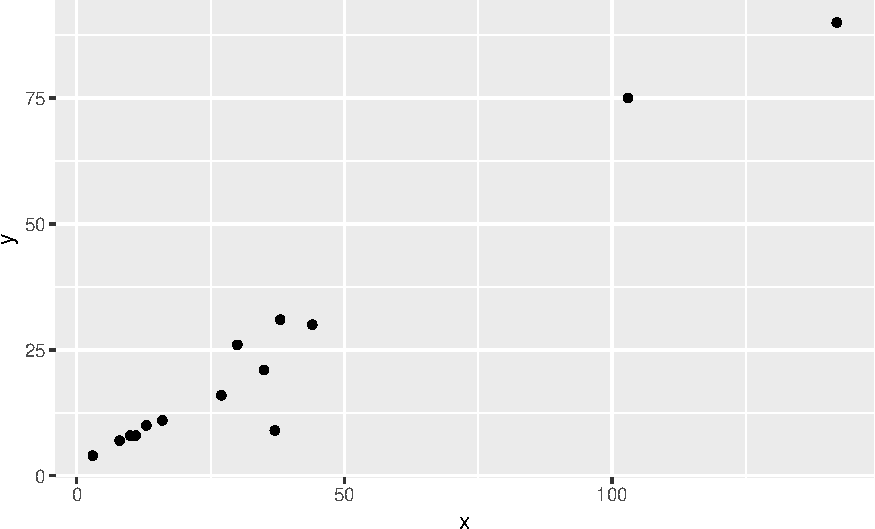
\includegraphics[width=0.7\linewidth]{regression-analysis_files/figure-latex/unnamed-chunk-3-1} \end{center}

Looking just with the eyes, we can see the linear relationship. Regression analysis estimates the relationship statistically.

\begin{Shaded}
\begin{Highlighting}[]
\NormalTok{BioOxyDemand }\OperatorTok\StringTok{ }
\StringTok{  }\KeywordTok{ggplot}\NormalTok{(}\KeywordTok{aes}\NormalTok{(x, y)) }\OperatorTok{+}
\StringTok{  }\KeywordTok{geom_smooth}\NormalTok{(}\DataTypeTok{method =} \StringTok{"lm"}\NormalTok{) }\OperatorTok{+}
\StringTok{  }\KeywordTok{geom_point}\NormalTok{()}
\end{Highlighting}
\end{Shaded}

\begin{center}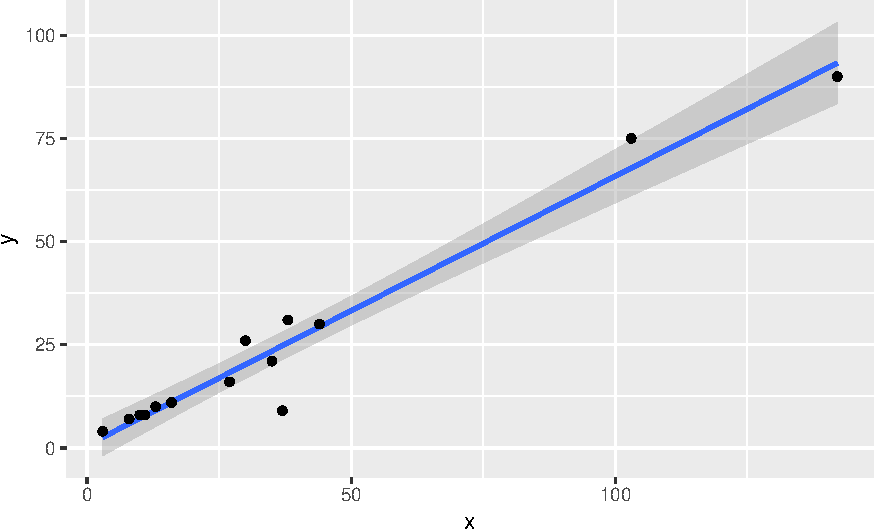
\includegraphics[width=0.7\linewidth]{regression-analysis_files/figure-latex/unnamed-chunk-4-1} \end{center}

\hypertarget{simple}{%
\chapter{Simple Linear Regression}\label{simple}}

\hypertarget{model}{%
\section{Model}\label{model}}

\begin{Shaded}
\begin{Highlighting}[]
\NormalTok{delv <-}\StringTok{ }\NormalTok{MPV}\OperatorTok{::}\NormalTok{p2}\FloatTok{.9} \OperatorTok\StringTok{ }\KeywordTok{tbl_df}\NormalTok{()}
\end{Highlighting}
\end{Shaded}

\begin{Shaded}
\begin{Highlighting}[]
\NormalTok{delv }\OperatorTok\StringTok{ }
\StringTok{  }\KeywordTok{ggplot}\NormalTok{(}\KeywordTok{aes}\NormalTok{(}\DataTypeTok{x =}\NormalTok{ x, }\DataTypeTok{y =}\NormalTok{ y)) }\OperatorTok{+}
\StringTok{  }\KeywordTok{geom_point}\NormalTok{() }\OperatorTok{+}
\StringTok{  }\KeywordTok{labs}\NormalTok{(}
    \DataTypeTok{x =} \StringTok{"Number of Cases"}\NormalTok{,}
    \DataTypeTok{y =} \StringTok{"Delivery Time"}
\NormalTok{  )}
\end{Highlighting}
\end{Shaded}

\begin{figure}[H]

{\centering 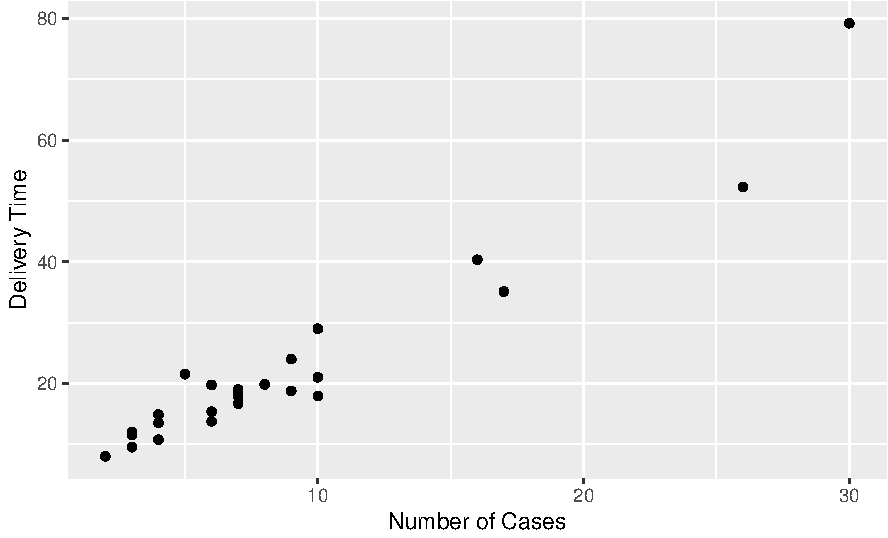
\includegraphics[width=0.7\linewidth]{regression-analysis_files/figure-latex/delivery-1} 

}

\caption{The Delivery Time Data\label{fig:delivery}}\label{fig:delivery}
\end{figure}

Given data \((x_1, Y_1), \ldots, (x_n, Y_n)\), we try to fit linear model

\[Y_i = \beta_0 + \beta_1 x_i + \epsilon_i\]

Here \(\epsilon_i\) is a error term, which is a random variable.

\[\epsilon \stackrel{iid}{\sim} (0, \sigma^2)\]

It gives the problem of estimating three parameters \((\beta_0, \beta_1, \sigma^2)\). Before estimating these, we set some assumptions.

\begin{enumerate}
\def\labelenumi{\arabic{enumi}.}
\tightlist
\item
  linear relationship
\item
  \(\epsilon_i\)s are independent
\item
  \(\epsilon_i\)s are identically destributed, i.e.~\emph{constant variance}
\item
  In some setting, \(\epsilon_i \sim N\)
\end{enumerate}

\hypertarget{least-squares-estimation}{%
\section{Least Squares Estimation}\label{least-squares-estimation}}

\begin{figure}[H]

{\centering 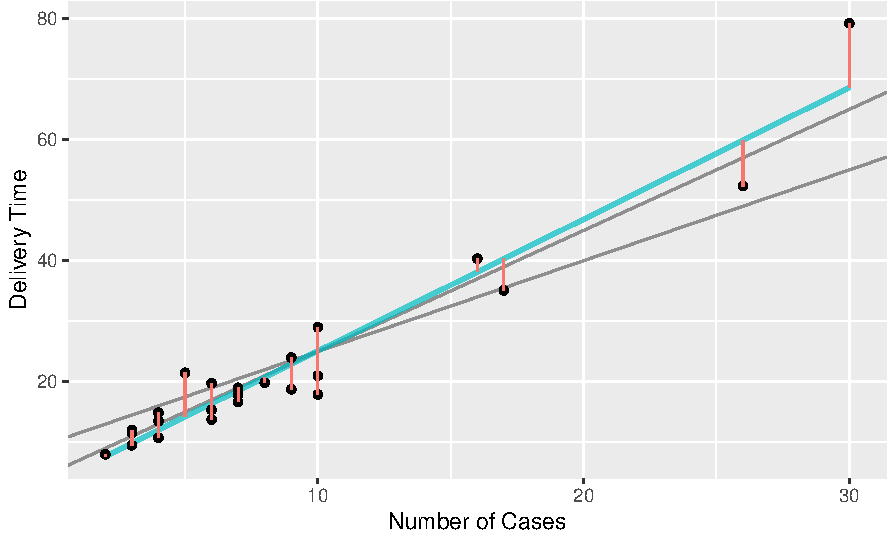
\includegraphics[width=0.7\linewidth]{regression-analysis_files/figure-latex/lsefig-1} 

}

\caption{Idea of the least square estimation\label{fig:lsefig}}\label{fig:lsefig}
\end{figure}

We try to find \(\beta_0\) and \(\beta_1\) that minimize the sum of squares of the vertical distances, i.e.

\begin{equation} \label{eq:ssq}
  (\beta_0, \beta_1) = \arg\min \sum_{i = 1}^n (Y_i - \beta_0 - \beta_1 x_i)^2
\end{equation}

\hypertarget{normal-equations}{%
\subsection{Normal equations}\label{normal-equations}}

Denote that Equation \(\eqref{eq:ssq}\) is quadratic. Then we can find its minimum by find the zero point of the first derivative. Set

\[Q(\beta_0, \beta_1) := \sum_{i = 1}^n (Y_i - \beta_0 - \beta_1 x_i)^2\]

Then we have

\begin{equation} \label{eq:normbeta0}
  \frac{\partial Q}{\partial \beta_0} = -2 \sum_{i = 1}^n(Y_i - \beta_0 - \beta_1 x_i) = 0
\end{equation}

and

\begin{equation} \label{eq:normbeta1}
  \frac{\partial Q}{\partial \beta_1} = -2 \sum_{i = 1}^n (Y_i - \beta_0 - \beta_1 x_i)x_i = 0
\end{equation}

From \(\eqref{eq:normbeta0}\),

\[\sum_{i = 1}^n Y_i - n \hat\beta_0 - \hat\beta_1 \sum_{i = 1}^n x_i = 0\]

Thus,

\[\hat\beta_0 = \overline{Y} - \hat\beta_1 \overline{x}\]

\(\eqref{eq:normbeta1}\) gives

\[\sum_{i = 1}^n x_i (Y_i - \overline{Y} + \hat\beta_1\overline{x} - \hat\beta_1 x_i) = \sum_{i = 1}^n x_i(Y_i - \overline{Y}) - \hat\beta_1\sum_{i = 1}^n x_i (x_i - \overline{x}) = 0\]

Thus,

\[\hat\beta_1 = \frac{\sum\limits_{i = 1}^nx_i(Y_i - \overline{Y})}{\sum\limits_{i = 1}^n x_i (x_i - \overline{x})}\]

\BeginKnitrBlock{remark}
\iffalse{} {Remark. } \fi{}\[\hat\beta_1 = \frac{S_{XY}}{S_{XX}}\]

where \(S_{XX} := \sum\limits_{i = 1}^n (x_i - \overline{x})^2\) and \(S_{XY} := \sum\limits_{i = 1}^n (x_i - \overline{x})(Y_i - \overline{Y})\)
\EndKnitrBlock{remark}

\BeginKnitrBlock{proof}
\iffalse{} {Proof. } \fi{}Note that \(\overline{x}^2 = \frac{1}{n^2}\bigg(\sum\limits_{i = 1}^n x_i\bigg)^2\). Then we have

\begin{equation} \label{eq:sxx}
  \begin{split}
    S_{XX} & = \sum_{i = 1}^n (x_i - \overline{x})^2 \\
    & = \sum_{i = 1}^n x_i^2 - 2\sum_{i = 1}^n x_i \overline{x} + \sum_{i = 1}^n\overline{x}^2 \\
    & = \sum_{i = 1}^n x_i^2 - \frac{2}{n}\bigg(\sum\limits_{i = 1}^n x_i\bigg)^2 + \frac{1}{n}\bigg(\sum\limits_{i = 1}^n x_i\bigg)^2 \\
    & = \sum_{i = 1}^n x_i^2 - \frac{1}{n}\bigg(\sum\limits_{i = 1}^n x_i\bigg)^2
  \end{split}
\end{equation}

It follows that

\begin{equation*}
  \begin{split}
    \hat\beta_1 & = \frac{\sum x_i(Y_i - \overline{Y})}{\sum x_i (x_i - \overline{x})} \\
    & = \frac{\sum x_i (Y_i - \overline{Y}) - \overline{x}\sum (Y_i - \overline{Y})}{\sum x_i^2 - \frac{1}{n} (\sum x_i)^2} \qquad \because \sum (Y_i - \overline{Y}) = 0 \\
    & = \frac{\sum (x_i - \overline{x})(Y_i - \overline{Y})}{\sum x_i^2 - \frac{1}{n} (\sum x_i)^2} \\
    & = \frac{S_{XY}}{S_{XX}}
  \end{split}
\end{equation*}
\EndKnitrBlock{proof}

\begin{Shaded}
\begin{Highlighting}[]
\KeywordTok{lm}\NormalTok{(y }\OperatorTok{~}\StringTok{ }\NormalTok{x, }\DataTypeTok{data =}\NormalTok{ delv)}
\end{Highlighting}
\end{Shaded}

\begin{verbatim}

Call:
lm(formula = y ~ x, data = delv)

Coefficients:
(Intercept)            x  
       3.32         2.18  
\end{verbatim}

\hypertarget{prediction-and-mean-response}{%
\subsection{Prediction and Mean response}\label{prediction-and-mean-response}}

\begin{quote}
``Essentially, all models are wrong, but some are useful.''

---George Box
\end{quote}

Recall that we have assumed the \textbf{linear assumption} between the predictor and the response variables, i.e.~the true model. Estimating \(\beta_0\) and \(\beta_1\) is same as estimating the \emph{assumed true model}.

\BeginKnitrBlock{definition}[Mean response]
\protect\hypertarget{def:eyx}{}{\label{def:eyx} \iffalse (Mean response) \fi{} }\[E(Y \mid X = x) = \beta_0 + \beta_1 x\]
\EndKnitrBlock{definition}

We can estimate this mean resonse by

\begin{equation} \label{eq:meanres}
  \widehat{E(Y \mid x)} = \hat\beta_0 + \hat\beta_1 x
\end{equation}

However, in practice, the model might not be true, which is included in \(\epsilon\) term.

\[Y_i = \beta_0 + \beta_1 x_i + \epsilon_i\]

Our real problem is predicting individual \(Y\), not the mean. The \emph{prediction} of response can be done by

\begin{equation} \label{eq:indpred}
  \hat{Y_i}  = \hat\beta_0 + \hat\beta_1 x_i
\end{equation}

Observe that the values of Equation \(\eqref{eq:meanres}\) and \(\eqref{eq:indpred}\) are same. However, due to the \textbf{error term in the prediction}, it has larger standard error.

\hypertarget{lseprop}{%
\subsection{Properties of LSE}\label{lseprop}}

Parameters \(\beta_0\) and \(\beta_1\) have some properties related to the expectation and variance. We can notice that these lse's are \textbf{unbiased linear estimator}. In fact, these are the \emph{best unbiased linear estimator}. This will be covered in the Gauss-Markov theorem.

\BeginKnitrBlock{lemma}
\protect\hypertarget{lem:sxy}{}{\label{lem:sxy} }\[S_{XX} = \sum_{i = 1}^n x_i^2 - \frac{1}{n}\bigg(\sum\limits_{i = 1}^n x_i\bigg)^2 = \sum_{i = 1}^n x_i(x_i - \overline{x})\]

\[S_{XY} = \sum_{i = 1}^n x_i Y_i - \frac{1}{n}\bigg(\sum_{i = 1}^n x_i\bigg)\bigg(\sum_{i = 1}^n Y_i\bigg) = \sum_{i = 1}^n Y_i(x_i - \overline{x})\]
\EndKnitrBlock{lemma}

\BeginKnitrBlock{proof}
\iffalse{} {Proof. } \fi{}We already proven the first part of \(S_{XX}\). See the Equation \(\eqref{eq:sxx}\). The second part is tivial. Since \(\sum (x_i - \overline{x}) = 0\),

\[S_{XX} = \sum_{i = 1}^n (x_i - \overline{x})^2 = \sum_{i = 1}^n (x_i - \overline{x})x_i\]

For the first part of \(S_{XY}\),

\begin{equation*}
  \begin{split}
    S_{XY} & = \sum_{i = 1}^n (x_i - \overline{x})(Y_i - \overline{Y}) \\
    & = \sum_{i = 1}^n x_i Y_i - \overline{x} \sum_{i = 1}^n Y_i - \overline{Y} \sum_{i = 1}^n x_i + n \overline{x} \overline{Y} \\
    & = \sum_{i = 1}^n x_i Y_i - \frac{1}{n}\bigg(\sum_{i = 1}^n x_i\bigg)\bigg(\sum_{i = 1}^n Y_i\bigg)
  \end{split}
\end{equation*}

Second part of \(S_{XY}\) also can be proven from the definition.

\begin{equation*}
  \begin{split}
    S_{XY} & = \sum_{i = 1}^n (x_i - \overline{x})(Y_i - \overline{Y}) \\
    & = \sum_{i = 1}^n Y_i (x_i - \overline{x}) - \overline{Y} \sum_{i = 1}^n (x_i - \overline{x}) \\
    & = \sum_{i = 1}^n Y_i (x_i - \overline{x}) \qquad \because \sum_{i = 1}^n (x_i - \overline{x}) = 0
  \end{split}
\end{equation*}
\EndKnitrBlock{proof}

\BeginKnitrBlock{lemma}[Linearity]
\protect\hypertarget{lem:linbet}{}{\label{lem:linbet} \iffalse (Linearity) \fi{} }Each coefficient is a linear estimator.

\[\hat\beta_1 = \sum_{i = 1}^n\frac{(x_i - \overline{x})}{S_{XX}}Y_i\]

\[\hat\beta_0 = \sum_{i = 1}^n \bigg( \frac{1}{n} - \frac{(x_i - \overline{x})}{S_{XX}} \bigg) Y_i\]
\EndKnitrBlock{lemma}

\BeginKnitrBlock{proof}
\iffalse{} {Proof. } \fi{}From lemma \ref{lem:sxy},

\begin{equation*}
  \begin{split}
    \hat\beta_1 & = \frac{S_{XY}}{S_{XX}} \\
    & = \frac{1}{S_{XX}}\sum_{i = 1}^n (x_i - \overline{x}) Y_i
  \end{split}
\end{equation*}

It gives that

\begin{equation*}
  \begin{split}
    \hat\beta_0 & = \overline{Y} - \hat\beta_1 \overline{x} \\
    & = \frac{1}{n}\sum_{i = 1}^n Y_i - \overline{x} \sum_{i = 1}^n\frac{(x_i - \overline{x})}{S_{XX}}Y_i \\
    & = \sum_{i = 1}^n\bigg(\frac{1}{n} - \frac{(x_i - \overline{x})\overline{x}}{S_{XX}} \bigg)Y_i
  \end{split}
\end{equation*}
\EndKnitrBlock{proof}

\BeginKnitrBlock{proposition}[Unbiasedness]
\protect\hypertarget{prp:ue}{}{\label{prp:ue} \iffalse (Unbiasedness) \fi{} }Both coefficients are unbiased.

\(\text{(a)}\: E\hat\beta_1 = \beta_1\)

\(\text{(b)}\: E\hat\beta_0 = \beta_0\)
\EndKnitrBlock{proposition}

From the model, \(Y_1, \ldots, Y_n \stackrel{indep}{\sim} (\beta_0 + \beta_1 x_i, \sigma^2)\).

\BeginKnitrBlock{proof}
\iffalse{} {Proof. } \fi{}From lemma \ref{lem:sxy},

\begin{equation*}
  \begin{split}
    E\hat\beta_1 & = \sum_{i = 1}^n \bigg[ \frac{(x_i - \overline{x})}{S_{XX}} E(Y_i) \bigg] \\
    & = \sum_{i = 1}^n \frac{(x_i - \overline{x})}{S_{XX}}(\beta_0 + \beta_1 x_i) \\
    & = \frac{\beta_1 \sum (x_i - \overline{x})x_i}{\sum (x_i - \overline{x})x_i} \qquad \because \sum (x_i - \overline{x}) = 0 \\
    & = \beta_1
  \end{split}
\end{equation*}

It follows that

\begin{equation*}
  \begin{split}
    E\hat\beta_0 & = E(\overline{Y} - \hat\beta_1 \overline{x}) \\
    & = E(\overline{Y}) - \overline{x}E(\hat\beta_1) \\
    & = E(\beta_0 + \beta_1 \overline{x} + \overline{\epsilon}) - \beta_1 \overline{x} \\
    & = \beta_0 + \beta_1 \overline{x} - \beta_1 \overline{x} \\
    & = \beta_0
  \end{split}
\end{equation*}
\EndKnitrBlock{proof}

\BeginKnitrBlock{proposition}[Variances]
\protect\hypertarget{prp:vb}{}{\label{prp:vb} \iffalse (Variances) \fi{} }Variances and covariance of coefficients

\(\text{(a)}\: Var\hat\beta_1 = \frac{\sigma^2}{S_{XX}}\)

\(\text{(b)}\: Var\hat\beta_0 = \bigg( \frac{1}{n} + \frac{\overline{x}^2}{S_{XX}} \bigg)\sigma^2\)

\(\text{(c)}\: Cov(\hat\beta_0, \hat\beta_1) = - \frac{\overline{x}}{S_{XX}} \sigma^2\)
\EndKnitrBlock{proposition}

\BeginKnitrBlock{proof}
\iffalse{} {Proof. } \fi{}Proving is just arithmetic.

\begin{enumerate}
\def\labelenumi{(\alph{enumi})}
\item
\end{enumerate}

\begin{equation*}
  \begin{split}
    Var\hat\beta_1 & = \frac{1}{S_{XX}^2}\sum_{i = 1}^n \bigg[ (x_i - \overline{x})^2 Var(Y_i) \bigg] + \frac{1}{S_{XX}^2} \sum_{j \neq k}^n \bigg[ (x_j - \overline{x})(x_k - \overline{x}) Cov(Y_j, Y_k) \bigg] \\
    & = \frac{\sigma^2}{S_{XX}} \qquad \because Cov(Y_j, Y_k) = 0 \: \text{if} \: j \neq k
  \end{split}
\end{equation*}

\begin{enumerate}
\def\labelenumi{(\alph{enumi})}
\setcounter{enumi}{1}
\item
\end{enumerate}

\begin{equation*}
  \begin{split}
    Var\hat\beta_0 & = \sum_{i = 1}^n \bigg( \frac{1}{n} - \frac{(x_i - \overline{x})\overline{x}}{S_{XX}} \bigg)^2Var(Y_i) + \sum_{j \neq k} \bigg( \frac{1}{n} - \frac{(x_j - \overline{x})\overline{x}}{S_{XX}} \bigg)\bigg( \frac{1}{n} - \frac{(x_k - \overline{x})\overline{x}}{S_{XX}} \bigg) Cov(Y_j, Y_k) \\
    & = \frac{\sigma^2}{n} - 2 \sigma^2 \frac{\overline{x}}{S_{XX}} \sum_{i = 1}^n (x_i - \overline{x}) + \frac{\sigma^2 \overline{x}^2 \sum (x_i - \overline{x})^2}{S_{XX}^2} \\
    & = \bigg( \frac{1}{n} + \frac{\overline{x}^2}{S_{XX}} \bigg) \sigma^2 \qquad \because \sum (x_i - \overline{x}) = 0
  \end{split}
\end{equation*}

\begin{enumerate}
\def\labelenumi{(\alph{enumi})}
\setcounter{enumi}{2}
\item
\end{enumerate}

\begin{equation*}
  \begin{split}
    Cov(\hat\beta_0, \hat\beta_1) & = Cov(\overline{Y} - \hat\beta_1 \overline{x}, \hat\beta_1) \\
    & = - \overline{x} Var\hat\beta_1 \\
    & = - \frac{\overline{x}}{S_{XX}} \sigma^2
  \end{split}
\end{equation*}
\EndKnitrBlock{proof}

\hypertarget{gauss-markov-theorem}{%
\subsection{Gauss-Markov Theorem}\label{gauss-markov-theorem}}

Chapter \ref{lseprop} shows that the \(\beta_0^{LSE}\) and \(\beta_1^{LSE}\) are the \textbf{linear unbiased estimators}. Are these good? Good compared to \emph{what estimators}? Here we consider \emph{linear unbiased estimator}. If variances in the proposition \ref{prp:vb} are lower than any parameters in this parameter family, \(\beta_0^{LSE}\) and \(\beta_1^{LSE}\) are the \textbf{best linear unbiased estimators}.

\BeginKnitrBlock{theorem}[Gauss Markov Theorem]
\protect\hypertarget{thm:gmt}{}{\label{thm:gmt} \iffalse (Gauss Markov Theorem) \fi{} }\(\hat\beta_0\) and \(\hat\beta_1\) are BLUE, i.e.~the best linear unbiased estimator.

\[Var(\hat\beta_0) \le Var\Big( \sum_{i = 1}^n a_i Y_i \Big) \: \forall a_i \in \mathbb{R} \: \text{s.t.} \: E\Big( \sum_{i = 1}^n a_i Y_i \Big) = \beta_0\]

\[Var(\hat\beta_1) \le Var\Big( \sum_{i = 1}^n b_i Y_i \Big) \: \forall b_i \in \mathbb{R} \: \text{s.t.} \: E\Big( \sum_{i = 1}^n b_i Y_i \Big) = \beta_1\]
\EndKnitrBlock{theorem}

\hypertarget{maximum-likelihood-estimation}{%
\section{Maximum Likelihood Estimation}\label{maximum-likelihood-estimation}}

In this section, we add an assumption to an random errors \(\epsilon_i\).

\[\epsilon_i \stackrel{iid}{\sim} N(0, \sigma^2)\]

\BeginKnitrBlock{example}[Gaussian Likelihood]
\protect\hypertarget{exm:gmle}{}{\label{exm:gmle} \iffalse (Gaussian Likelihood) \fi{} }Note that \(Y_i \stackrel{indep}{\sim} N(\beta_0 + \beta_1 x_i, \sigma^2)\). Then the likelihood function is

\[L(\beta_0, \beta_1, \sigma^2) = \prod_{i = 1}^n\bigg( \frac{1}{\sqrt{2\pi\sigma^2}} \exp \bigg(- \frac{(Y_i - \beta_0 - \beta_1 x_i)^2}{2 \sigma^2} \bigg) \bigg)\]

and so the log-likelihood function can be computed as

\[l(\beta_0, \beta_1, \sigma^2) = -\frac{n}{2}\ln(2\pi\sigma^2) - \frac{1}{2\sigma^2}\sum_{i = 1}^n(Y_i - \beta_0 - \beta_1 x_i)^2\]
\EndKnitrBlock{example}

\hypertarget{likelihood-equations}{%
\subsection{Likelihood equations}\label{likelihood-equations}}

\BeginKnitrBlock{definition}[Maximum Likelihood Estimator]
\protect\hypertarget{def:mledef}{}{\label{def:mledef} \iffalse (Maximum Likelihood Estimator) \fi{} }\[(\hat\beta_0^{MLE}, \hat\beta_1^{MLE}, \hat\sigma^{2MLE}) := \arg\sup L(\beta_0, \beta_1, \sigma^2)\]
\EndKnitrBlock{definition}

Since \(l(\cdot) = \ln L(\cdot)\) is monotone,

\BeginKnitrBlock{remark}
\iffalse{} {Remark. } \fi{}\[(\hat\beta_0^{MLE}, \hat\beta_1^{MLE}, \hat\sigma^{2MLE}) = \arg\sup l(\beta_0, \beta_1, \sigma^2)\]
\EndKnitrBlock{remark}

We can find the maximum of this \emph{quadratic} function by making first derivative.

\begin{equation} \label{eq:mlbeta0}
  \frac{\partial l}{\partial \beta_0} = \frac{1}{\sigma^2} \sum_{i = 1}^n (Y_i - \beta_0 - \beta_1 x_i) = 0
\end{equation}

\begin{equation} \label{eq:mlbeta1}
  \frac{\partial l}{\partial \beta_1} = \frac{1}{\sigma^2} \sum_{i = 1}^n x_i (Y_i - \beta_0 - \beta_1 x_i) = 0
\end{equation}

\begin{equation} \label{eq:mlsig}
  \frac{\partial l}{\partial \sigma^2} = - \frac{n}{2\sigma^2} + \frac{1}{2\sigma^4} \sum_{i = 1}^n (Y_i - \beta_0 - \beta_1 x_i)^2 = 0
\end{equation}

Denote that Equations \(\eqref{eq:mlbeta0}\) and \(\eqref{eq:mlbeta1}\) given \(\hat\sigma^2\) are equivalent to the normal equations. Thus,

\[\hat\beta_0^{MLE} = \hat\beta_0^{LSE}, \quad \hat\beta_1^{MLE} = \hat\beta_1^{LSE}\]

From \(\eqref{eq:mlsig}\),

\[\hat\sigma^{2MLE} = \frac{1}{n}\sum_{i = 1}^n(Y_i - \beta_0 - \beta_1 x_i)^2 = \frac{n - 2}{n} \hat\sigma^{2LSE}\]

Recall that \(\hat\sigma^{2LSE}\) is an unbiased, i.e.~this \emph{MLE is not an unbiased estimator}. Since \(\hat\sigma^{2MLE} \approx \hat\sigma^{2LSE}\) for large \(n\), howerver, it is \emph{asymptotically unbiased}.

\BeginKnitrBlock{theorem}[Rao-Cramer Lower Bound, univariate case]
\protect\hypertarget{thm:rclb}{}{\label{thm:rclb} \iffalse (Rao-Cramer Lower Bound, univariate case) \fi{} }Let \(X_1, \ldots, X_n \stackrel{iid}{\sim} f(x ; \theta)\). If \(\hat\theta\) is an unbiased estimator of \(\theta\),

\[Var(\hat\theta) \ge \frac{1}{I_n(\theta)}\]

where \(I_n(\theta) = -E\bigg(\frac{\partial^2 l(\theta)}{\partial \theta^2} \bigg)\)
\EndKnitrBlock{theorem}

To apply this theorem @(thm:rclb) in the simple linear regression setting, i.e.~\((\beta_0, \beta_1)\), we need to look at the \emph{bivariate case}.

\BeginKnitrBlock{theorem}[Rao-Cramer Lower Bound, bivariate case]
\protect\hypertarget{thm:rclb2}{}{\label{thm:rclb2} \iffalse (Rao-Cramer Lower Bound, bivariate case) \fi{} }Let \(X_1, \ldots, X_n \stackrel{iid}{\sim} f(x ; \theta1, \theta_2)\) and let \(\boldsymbol{\theta} = (\theta_1, \theta_2)^T\). If each \(\hat\theta_1\), \(\hat\theta_2\) is an unbiased estimator of \(\theta_1\) and \(\theta_2\), then

\[
Var(\boldsymbol{\theta}) := \begin{bmatrix}
Var(\hat\theta_1) & Cov(\hat\theta_1, \hat\theta_2) \\
Cov(\hat\theta_1, \hat\theta_2) & Var(\hat\theta_2)
\end{bmatrix} \ge I_n^{-1}(\theta_1, \theta_2)
\]

where

\[
I_n(\theta_1, \theta_2) = - \begin{bmatrix}
  E\bigg( \frac{\partial^2 l(\theta_1, \theta_2)}{\partial \theta_1^2} \bigg) & E\bigg( \frac{\partial^2 l(\theta_1, \theta_2)}{\partial \theta_1 \partial \theta_2} \bigg) \\
  E\bigg( \frac{\partial^2 l(\theta_1, \theta_2)}{\partial \theta_1 \partial \theta_2} \bigg) & E\bigg( \frac{\partial^2 l(\theta_1, \theta_2)}{\partial \theta_2^2} \bigg)
\end{bmatrix}
\]
\EndKnitrBlock{theorem}

\hypertarget{references}{%
\chapter*{References}\label{references}}
\addcontentsline{toc}{chapter}{References}

\bibliography{book.bib,packages.bib}


\end{document}
